\documentclass[11pt,a4paper]{report}

\usepackage[utf8]{inputenc}
\usepackage[T1]{fontenc}
\usepackage[english]{babel}
\usepackage{geometry}
\usepackage{graphicx}
\usepackage{array}
\usepackage{booktabs}
\usepackage{float}
\usepackage{xcolor}
\usepackage{hyperref}
\usepackage{listings}
\usepackage{caption}
\usepackage{amsmath}
\usepackage{enumitem}
\usepackage{tabularx}
\usepackage{titlesec}
\usepackage{fancyhdr}
\usepackage{setspace}
\graphicspath{{../metrics/}{metrics/}{../assets/figures/}{assets/figures/}{./}}

\geometry{margin=2cm}
\setstretch{0.94}
\setlist{nosep}
\hypersetup{
    colorlinks=true,
    linkcolor=black,
    urlcolor=blue
}

% ─── Python code style ────────────────────────────────────────────────────────
\lstdefinestyle{pythonStyle}{
    language=Python,
    basicstyle=\ttfamily\small,
    keywordstyle=\color{blue!70!black}\bfseries,
    stringstyle=\color{green!40!black},
    commentstyle=\color{gray}\itshape,
    numbers=left,
    numberstyle=\tiny\color{gray},
    stepnumber=1,
    numbersep=8pt,
    frame=single,
    breaklines=true,
    tabsize=4,
    captionpos=b,
    showstringspaces=false
}

% ─── JSON / shell style ───────────────────────────────────────────────────────
\lstdefinestyle{jsonStyle}{
    basicstyle=\ttfamily\small,
    keywordstyle=\color{blue!70!black},
    stringstyle=\color{green!40!black},
    morestring=[b]",
    frame=single,
    breaklines=true,
    tabsize=2,
    captionpos=b,
    showstringspaces=false
}

% ─── Colour definitions ───────────────────────────────────────────────────────
\definecolor{droughtRed}{RGB}{220,38,38}
\definecolor{normalGreen}{RGB}{34,197,94}
\definecolor{accentBlue}{RGB}{59,130,246}
\definecolor{sectionGray}{RGB}{71,85,105}
\definecolor{chapterBlue}{RGB}{0,45,105}

\setlength{\headheight}{15pt}
\pagestyle{fancy}
\fancyhf{}
\fancyhead[L]{\textcolor{chapterBlue}{\textbf{Optimisation}}}
\fancyhead[R]{\textcolor{chapterBlue}{\textbf{2025--2026}}}
\fancyfoot[C]{\thepage}
\renewcommand{\headrulewidth}{0.5pt}
\renewcommand{\footrulewidth}{0.5pt}

\fancypagestyle{plain}{
    \fancyhf{}
    \fancyhead[L]{\textcolor{chapterBlue}{\textbf{Optimisation}}}
    \fancyhead[R]{\textcolor{chapterBlue}{\textbf{2025--2026}}}
    \fancyfoot[C]{\thepage}
    \renewcommand{\headrulewidth}{0.5pt}
    \renewcommand{\footrulewidth}{0.5pt}
}

\titleclass{\chapter}{straight}
\titleformat{\chapter}[display]
  {\normalfont\huge\bfseries}
  {\color{chapterBlue}\chaptertitlename\ \thechapter}
  {10pt}
  {\Huge\bfseries}
\titlespacing*{\chapter}{0pt}{-10pt}{20pt}
\titlespacing*{\section}{0pt}{8pt}{5pt}

\begin{document}

% ══════════════════════════════════════════════════════════════════════════════
%  TITLE PAGE
% ══════════════════════════════════════════════════════════════════════════════
\begin{titlepage}
    \centering
    \vspace*{0.5cm}

    \includegraphics[width=0.42\textwidth]{logo_university.png}\\[1cm]

    {\Large \textbf{Faculté des Sciences Ben M'Sik}}\\[0.3cm]
    {\large Université Hassan II de Casablanca}\\[2cm]

    {\Huge \textbf{Academic Project Report}}\\[0.4cm]
    {\LARGE Excellence Master Artificial Intelligence}\\[1.5cm]

    \rule{0.85\textwidth}{0.5pt}\\[0.4cm]
    {\Large \textbf{Optimization and Compression of Small Language Models\\[0.2cm]
    for Edge AI Applications}}\\[0.3cm]
    {\large \textit{Light tuning instructions: adapt an SLM by following simple instructions}}\\[0.4cm]
    \rule{0.85\textwidth}{0.5pt}

    \vfill

    \begin{tabular}{l@{\hskip 6cm}l}
        \textbf{Prepared by}  & \textbf{Supervisor}       \\[0.3cm]
        Othman Salahi         & Pr. Benabbou Faouzia      \\
        Aymene Chouki         &                           \\
        Malak Houali          &                           \\
        Hiba Dellaji          &                           \\
    \end{tabular}

    \vfill

     \begin{center}
        \normalsize{Course:} Optimisation\\[0.3cm]
        \normalsize{Academic year:} 2025--2026
    \end{center}

\end{titlepage}

\pagenumbering{arabic}
\tableofcontents
\clearpage
\listoffigures
\newpage

\chapter*{Abstract}
\addcontentsline{toc}{chapter}{Abstract}

\vspace*{2cm}


This project focuses on the optimization and compression of Small Language Models
for Edge AI applications. The main objective is to prepare and fine-tune a compact
instruction-following language model, \texttt{google/flan-t5-small}, and to study
the impact of different optimization algorithms on training quality and resource
efficiency.

\vspace*{0.15cm}

The dataset used in this work is \texttt{yahma/alpaca-cleaned}, which was processed
into training, validation, and test subsets. Each example was transformed into an
instruction-tuning format composed of a source prompt and a target answer. The
fine-tuning pipeline was then designed to train the model using several optimizers,
including Stochastic Gradient Descent, SGD with momentum, Adam, and L-BFGS. Newton-CG
is also discussed from a theoretical perspective because it is not practical for
standard transformer fine-tuning in this context.

\vspace*{0.15cm}

The comparison is based on criteria that are important for Edge AI deployment:
validation loss, perplexity, training time, training speed, memory consumption,
model size, inference time, latency, and energy consumption when power telemetry is
available. These metrics make it possible to analyze the tradeoff between model
quality and computational efficiency.

\vspace*{0.15cm}

This report presents the project context, the data preparation process, the
fine-tuning methodology, the optimization algorithms studied, and the evaluation
strategy. The final goal is to identify which optimization approach provides the
best compromise for adapting a Small Language Model under the constraints of Edge
AI environments.


\clearpage
\chapter*{List of Abbreviations}
\addcontentsline{toc}{chapter}{List of Abbreviations}

\vspace*{1cm}

\begin{tabularx}{\textwidth}{>{\bfseries}l X}
AI & Artificial Intelligence \\
SLM & Small Language Model \\
LLM & Large Language Model \\
NLP & Natural Language Processing \\
Edge AI & Artificial Intelligence executed directly on edge devices \\
GPU & Graphics Processing Unit \\
CPU & Central Processing Unit \\
CUDA & Compute Unified Device Architecture \\
SGD & Stochastic Gradient Descent \\
L-BFGS & Limited-memory Broyden-Fletcher-Goldfarb-Shanno algorithm \\
Newton-CG & Newton Conjugate Gradient method \\
FLAN-T5 & Fine-tuned Language Net Text-to-Text Transfer Transformer \\
CSV & Comma-Separated Values \\
JSONL & JSON Lines \\
RAM & Random Access Memory \\
\end{tabularx}


\clearpage
\chapter{Context and Objectives}

\vspace*{0.3cm}

Artificial Intelligence has become an important technology in modern applications,
especially with the development of language models capable of understanding
instructions and generating natural language responses. However, large language
models require significant computation, memory, and energy, which makes their
deployment difficult on constrained devices. Edge AI addresses this limitation by
executing models directly on local devices such as embedded systems, sensors, or
small computing boards. This improves latency, autonomy, and privacy, but it also
requires models that are compact and efficient \cite{edgeai}.

Small Language Models are therefore useful because they provide language
capabilities with a lower computational cost than large models. In this project,
the selected model is \texttt{google/flan-t5-small}, a compact instruction-tuned
model from the T5 family \cite{flant5model}. T5 represents tasks in a
text-to-text format, which is well suited for instruction-following data
\cite{t5}. Fine-tuning is used to adapt this pre-trained model to the prepared
dataset instead of training a model from scratch.

The objective of this work is to study the optimization of a Small Language Model
for Edge AI applications. The project prepares an instruction-tuning dataset,
fine-tunes \texttt{google/flan-t5-small}, and compares several optimization
algorithms: SGD, SGD with momentum, Adam, AdamW with clipping and scheduling,
L-BFGS, and Newton-CG. The comparison is not based only on validation loss, but
also on training latency, inference latency, throughput, and GPU memory usage.
These criteria are essential because an Edge AI model must be accurate, fast, and
resource-efficient.

The work also prepares a baseline for future compression. Techniques such as
quantization, pruning, and knowledge distillation are not fully implemented in
this report, but the optimizer comparison helps identify which fine-tuned model
would be the best candidate for later compression experiments.


\chapter{Project and Data Preparation}

\vspace*{0.3cm}

The project workflow starts with the raw instruction-following dataset and ends
with optimizer comparison for Edge AI analysis. Figure~\ref{fig:project_workflow}
summarizes the full pipeline, including data preparation, instruction formatting,
model loading, fine-tuning, evaluation, and future compression analysis.

\begin{figure}[H]
    \centering
    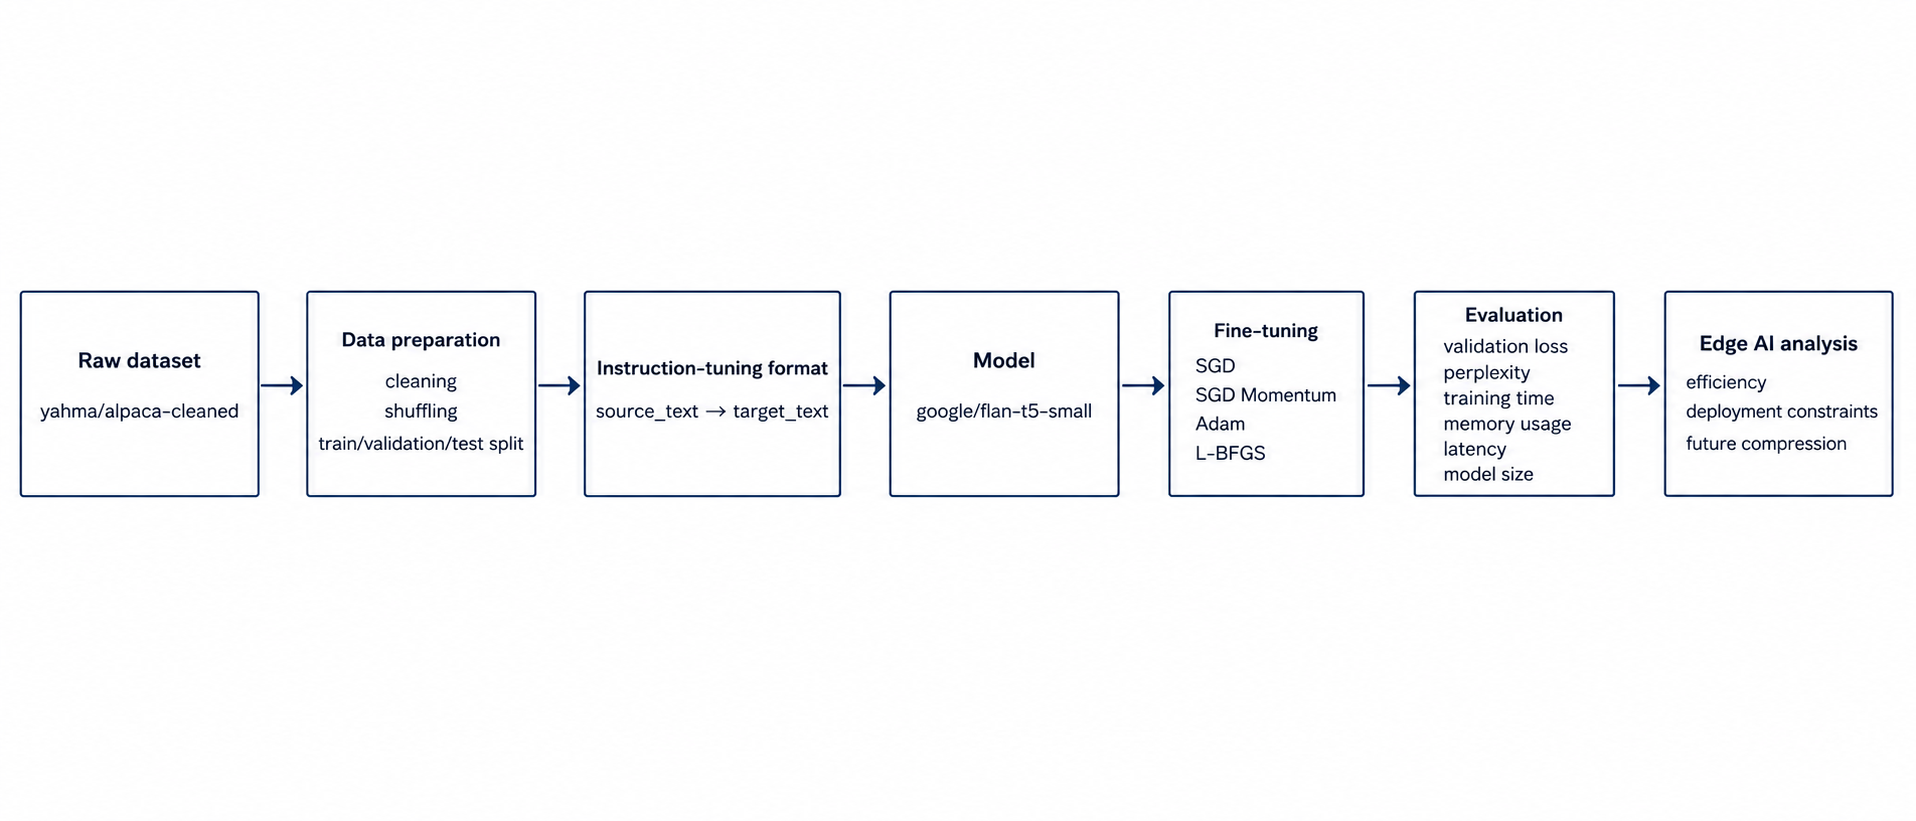
\includegraphics[width=\textwidth]{chapters/images/project_flow.png}
    \caption{General workflow of the project.}
    \label{fig:project_workflow}
\end{figure}

The dataset used is \texttt{yahma/alpaca-cleaned}, downloaded using the Hugging
Face \texttt{datasets} library \cite{alpaca}. Each example contains an
instruction, an optional input, and an output. This structure is appropriate for
instruction tuning because the model learns to generate an answer from a natural
language prompt. Figure~\ref{fig:dataset_examples} shows examples extracted from
the dataset.

\begin{figure}[H]
    \centering
    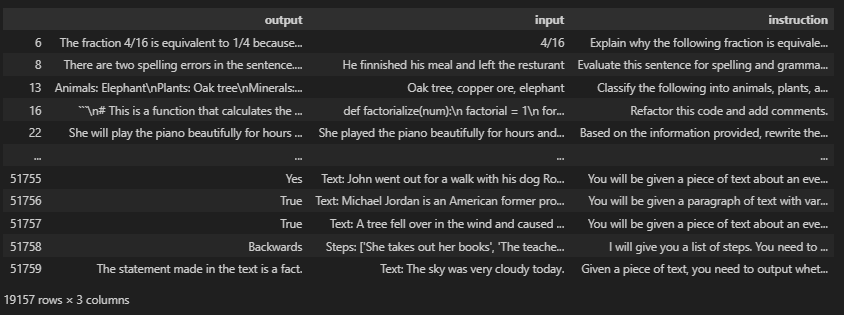
\includegraphics[width=0.95\textwidth]{chapters/images/dataset_examples.png}
    \caption{Examples extracted from the original instruction-following dataset.}
    \label{fig:dataset_examples}
\end{figure}

The data preparation configuration is stored in \texttt{config.yaml}. The
processed dataset contains 2000 training examples, 500 validation examples, and
500 test examples, with seed 42 for reproducibility. The processed files are
saved in \texttt{data/processed/} as \texttt{CSV} and \texttt{JSONL} files.

\begin{figure}[H]
    \centering
    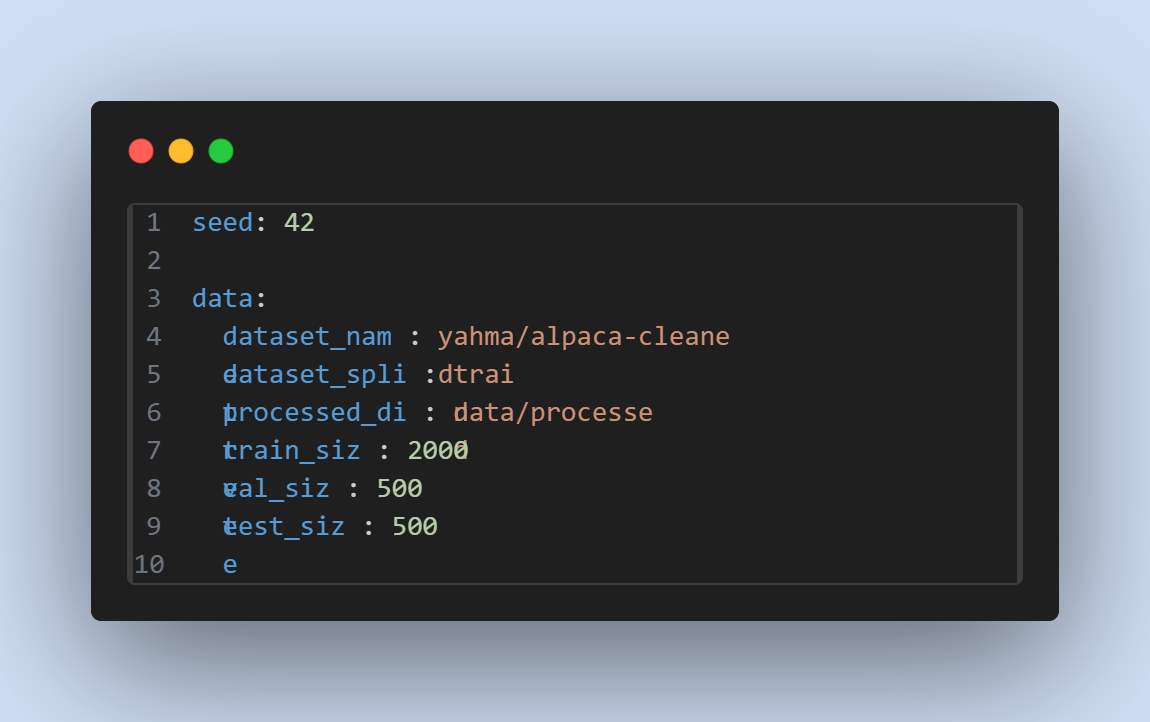
\includegraphics[width=0.8\textwidth]{chapters/images/config-yaml.png}
    \caption{Configuration file used for data preparation.}
    \label{fig:yaml_config}
\end{figure}

The preprocessing script \texttt{src/prepare\_data.py} loads the configuration,
downloads and shuffles the dataset, creates the train/validation/test subsets,
cleans empty fields, converts the data into instruction-tuning format, and saves
the processed files. The final model input is stored in \texttt{source\_text},
while the expected answer is stored in \texttt{target\_text}. If an example has
an input, the prompt contains the instruction, the input, and the keyword
\texttt{Answer:}. If no input is available, the prompt contains only the
instruction and \texttt{Answer:}.

\begin{figure}[H]
    \centering
    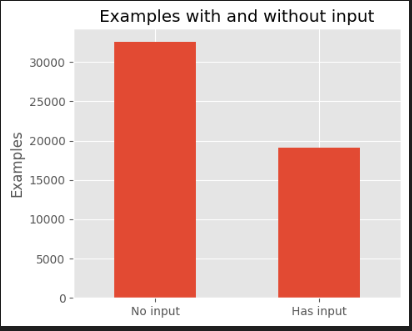
\includegraphics[width=0.5\textwidth]{chapters/images/input_distribution.png}
    \caption{Distribution of examples with and without input in the dataset.}
    \label{fig:input_distribution}
\end{figure}

\begin{table}[H]
    \centering
    \begin{tabular}{lr}
        \toprule
        \textbf{Statistic} & \textbf{Value} \\
        \midrule
        Original examples & 51760 \\
        Training examples & 2000 \\
        Validation examples & 500 \\
        Test examples & 500 \\
        Average source length & 17.14 words \\
        Average target length & 109.21 words \\
        Maximum source length & 279 words \\
        Maximum target length & 450 words \\
        \bottomrule
    \end{tabular}
    \caption{Statistics of the processed dataset.}
    \label{tab:data_stats}
\end{table}


\chapter{Fine-Tuning Methodology and Optimizers}

\vspace*{0.3cm}

The fine-tuning methodology adapts \texttt{google/flan-t5-small} \cite{flant5}
to the prepared
instruction-following dataset. The tokenizer converts \texttt{source\_text} and
\texttt{target\_text} into token IDs using padding and truncation. The training
script then loads the model, selects the optimizer, runs the training loop,
evaluates the model, and saves the metrics.

\begin{figure}[H]
    \centering
    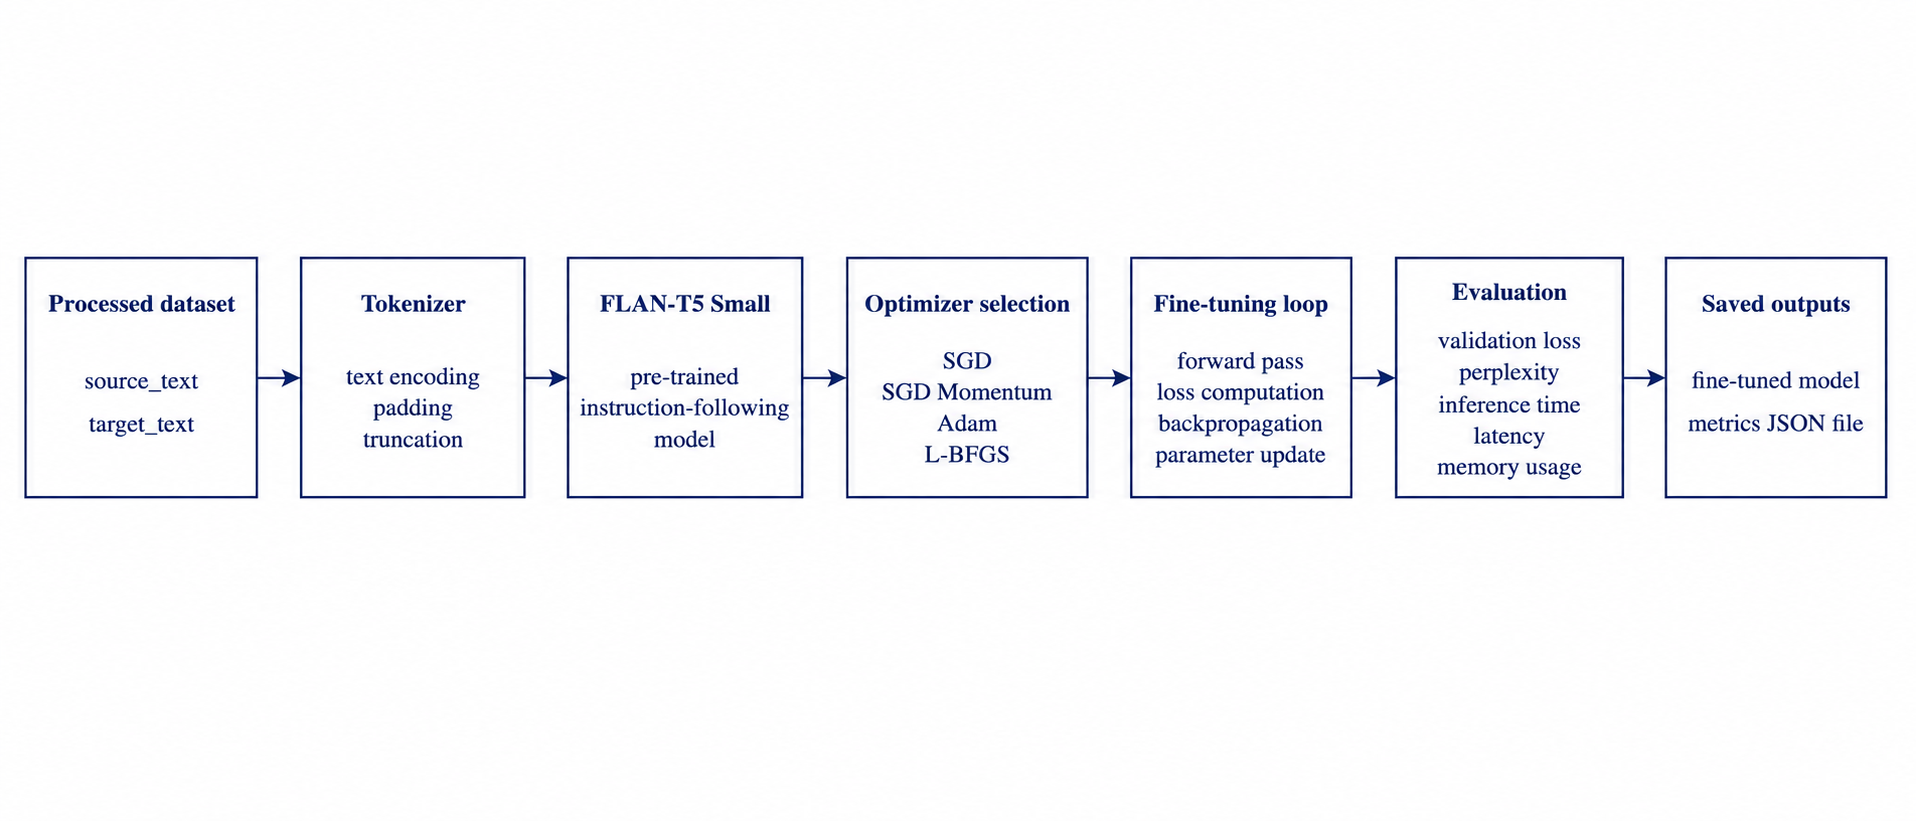
\includegraphics[width=\textwidth]{chapters/images/finetunning_flow.png}
    \caption{Fine-tuning workflow used in the project.}
    \label{fig:finetuning_workflow}
\end{figure}

The main implementation is organized around \texttt{src/train.py}, supported by
\texttt{model\_utils.py}, \texttt{tokenizer\_utils.py}, \texttt{optimizers.py},
\texttt{training\_config.py}, and \texttt{metrics.py}. The implementation relies
on the Hugging Face Transformers ecosystem \cite{transformers}. The experiments were run
on a CUDA-enabled GPU, specifically an RTX 5060. CPU execution is kept only for
debugging because it is too slow for complete optimizer comparison.

\begin{figure}[H]
    \centering
    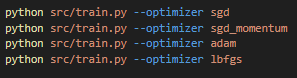
\includegraphics[width=0.5\textwidth]{chapters/images/optimizer_training_commands.png}
    \caption{Commands used to launch fine-tuning with each optimizer.}
    \label{fig:optimizer_training_commands}
\end{figure}

SGD is the simplest first-order method and updates parameters using the gradient
of the loss \cite{sgd}.

\[
\theta_{t+1} = \theta_t - \eta \nabla_{\theta} L(\theta_t)
\]

It is memory-efficient but can converge slowly. SGD with momentum improves this
method by accumulating part of the previous update direction, which reduces
oscillation and can accelerate convergence.

\[
v_{t+1} = \mu v_t + \nabla_{\theta}L(\theta_t), \quad \theta_{t+1} = \theta_t - \eta v_{t+1}
\]

Adam, or Adaptive Moment Estimation, combines momentum and adaptive learning
rates by maintaining moving averages of gradients and squared gradients. It is
widely used for transformer fine-tuning because it often reduces loss faster than
SGD \cite{adam}.

\[
m_t = \beta_1m_{t-1} + (1-\beta_1)g_t, \quad v_t = \beta_2v_{t-1} + (1-\beta_2)g_t^2, \quad \theta_{t+1} = \theta_t - \eta\frac{\hat{m}_t}{\sqrt{\hat{v}_t}+\epsilon}
\]

AdamW extends Adam by decoupling weight decay from the gradient
update, which can improve regularization \cite{adamw}.

\[
\theta_{t+1} = \theta_t - \eta\left(\frac{\hat{m}_t}{\sqrt{\hat{v}_t}+\epsilon} + \lambda\theta_t\right)
\]

L-BFGS is a quasi-Newton method that
approximates curvature information but is expensive for transformer models
\cite{lbfgs}.

\[
p_k = -H_k \nabla_{\theta}L(\theta_k), \quad \theta_{k+1} = \theta_k + \alpha_k p_k
\]

Newton-CG is a second-order method based on Hessian information; it is useful for
academic comparison but costly in practice.

\[
\theta_{t+1} = \theta_t - H^{-1}\nabla_{\theta}L(\theta_t)
\]

Each optimizer saves its own model under \texttt{results/models/} and its metrics
under \texttt{results/metrics/}. This makes the comparison reproducible and keeps
the outputs of each experiment separated.


\chapter{Evaluation and Experimental Results}

\vspace*{0.3cm}

The evaluation combines model quality and efficiency metrics. Validation loss
measures generalization on unseen data, while perplexity gives a language-modeling
interpretation of the loss. Efficiency is measured using training step latency,
inference latency, throughput, and peak VRAM usage. These metrics are important
because Edge AI models must be deployable under memory and latency constraints.

The benchmark was executed on a performant GPU using 10 training steps and a
batch size of 4. The tested configurations were inference-only baseline, SGD, SGD
with momentum, Adam, AdamW with clipping and scheduler, L-BFGS, and Newton-CG.
Figure~\ref{fig:optimizer_comparison_matrix} summarizes the complete comparison.

\begin{figure}[H]
    \centering
    
\includegraphics[width=\textwidth]{chapters/images/optimizer_comparison_matrix.png}
    \caption{Comparison matrix of the optimizer benchmark results.}
    \label{fig:optimizer_comparison_matrix}
\end{figure}

\begin{table}[H]
    \centering
    \scriptsize
    \begin{tabular}{lrrrrrr}
        \toprule
        \textbf{Optimizer} & \textbf{Train Loss} & \textbf{Val Loss} &
        \textbf{Step ms} & \textbf{Inf. ms} & \textbf{Tok/s} &
        \textbf{VRAM MB} \\
        \midrule
        Inference Only & 10.9235 & 10.8968 & 76.43 & 224.15 & 20096.52 & 553.23 \\
        SGD & 10.8635 & 10.8049 & 84.97 & 211.06 & 18076.50 & 1459.34 \\
        SGD + Momentum & 10.7055 & 10.5485 & 92.56 & 216.98 & 16595.08 & 1714.17 \\
        Adam & 9.4310 & 9.2548 & 190.80 & 1246.35 & 8050.34 & 1969.00 \\
        AdamW + Clip + Sched & 10.2606 & 10.0681 & 112.17 & 217.35 & 13693.65 & 1969.00 \\
        L-BFGS & 10.9365 & 10.8968 & 248.46 & 228.55 & 6182.03 & 5281.85 \\
        Newton-CG & 10.9030 & 10.1138 & 1445.42 & 1276.49 & 1062.67 & 6334.53 \\
        \bottomrule
    \end{tabular}
    \caption{Numerical summary of the optimizer benchmark.}
    \label{tab:benchmark_results}
\end{table}

Adam obtains the best model quality with a final training loss of 9.4310 and a
validation loss of 9.2548. SGD with momentum improves over plain SGD, reaching a
validation loss of 10.5485 compared with 10.8049 for SGD. AdamW with clipping and
scheduling gives an intermediate result, with better quality than SGD but better
efficiency than Adam.

From an efficiency perspective, SGD is the fastest trained optimizer, with 84.97
ms per step, 211.06 ms inference latency, and 18076.50 tokens per second. SGD
with momentum remains efficient, while Adam is slower and shows high inference
latency. L-BFGS and Newton-CG are the least practical methods because they require
high VRAM and have much higher training latency. Newton-CG reaches 6334.53 MB of
VRAM and 1445.42 ms per step, which is not suitable for Edge AI constraints.


\chapter{Discussion and Conclusion}

\vspace*{0.3cm}

The results show a clear tradeoff between model quality and computational
efficiency. Adam is the best optimizer for reducing training and validation loss,
which makes it the strongest quality baseline. However, it is slower than
SGD-based methods and has higher inference latency. For Edge AI, the best
optimizer is not necessarily the one with the lowest loss, because deployment
also depends on latency, throughput, memory usage, and model size.

SGD gives the best efficiency among the trained optimizers, while SGD with
momentum improves the validation loss with only a moderate increase in cost.
AdamW with clipping and scheduling is also a useful compromise because it gives
better quality than SGD while remaining more efficient than Adam. L-BFGS and
Newton-CG are important from an optimization theory perspective, but their high
memory and computational costs make them less practical for transformer
fine-tuning in an Edge AI context.

The project has several limitations. The dataset is intentionally small, with
2000 training examples and 500 validation/test examples. The benchmark is also
short, using only 10 training steps and a batch size of 4, so it compares early
optimizer behavior rather than complete convergence. The results also depend on
the GPU used during execution, and energy consumption could not be fully analyzed
without reliable power telemetry.

Overall, the project demonstrates that optimizer selection must be guided by the
target objective. Adam should be selected when fine-tuning quality is the main
priority. SGD with momentum or AdamW are better candidates when the objective is
to balance quality and efficiency for Edge AI deployment. The results provide a
baseline for future compression techniques such as quantization, pruning, and
knowledge distillation, which can further reduce memory usage and latency while
preserving acceptable model quality.


\begin{thebibliography}{99}

\bibitem{flant5}
H. W. Chung, L. Hou, S. Longpre, B. Zoph, Y. Tay, W. Fedus, E. Li, X. Wang,
M. Dehghani, S. Brahma, A. Webson, S. S. Gu, Z. Dai, M. Suzgun, X. Chen,
A. Chowdhery, A. Castro-Ros, M. Pellat, K. Robinson, D. Valter, S. Narang,
G. Mishra, A. Yu, V. Zhao, Y. Huang, A. Dai, H. Yu, S. Petrov, E. H. Chi,
J. Dean, J. Devlin, A. Roberts, D. Zhou, Q. V. Le, and J. Wei,
\textit{Scaling Instruction-Finetuned Language Models},
arXiv preprint arXiv:2210.11416, 2022.

\bibitem{t5}
C. Raffel, N. Shazeer, A. Roberts, K. Lee, S. Narang, M. Matena,
Y. Zhou, W. Li, and P. J. Liu,
\textit{Exploring the Limits of Transfer Learning with a Unified Text-to-Text Transformer},
Journal of Machine Learning Research, vol. 21, no. 140, pp. 1--67, 2020.

\bibitem{adam}
D. P. Kingma and J. Ba,
\textit{Adam: A Method for Stochastic Optimization},
International Conference on Learning Representations, 2015.

\bibitem{adamw}
I. Loshchilov and F. Hutter,
\textit{Decoupled Weight Decay Regularization},
International Conference on Learning Representations, 2019.

\bibitem{lbfgs}
D. C. Liu and J. Nocedal,
\textit{On the Limited Memory BFGS Method for Large Scale Optimization},
Mathematical Programming, vol. 45, pp. 503--528, 1989.

\bibitem{sgd}
L. Bottou,
\textit{Large-Scale Machine Learning with Stochastic Gradient Descent},
Proceedings of COMPSTAT, pp. 177--186, 2010.

\bibitem{transformers}
T. Wolf, L. Debut, V. Sanh, J. Chaumond, C. Delangue, A. Moi,
P. Cistac, T. Rault, R. Louf, M. Funtowicz, J. Davison, S. Shleifer,
P. von Platen, C. Ma, Y. Jernite, J. Plu, C. Xu, T. Le Scao, S. Gugger,
M. Drame, Q. Lhoest, and A. Rush,
\textit{Transformers: State-of-the-Art Natural Language Processing},
Proceedings of the 2020 Conference on Empirical Methods in Natural Language
Processing: System Demonstrations, pp. 38--45, 2020.

\bibitem{edgeai}
X. Wang, Y. Han, V. C. M. Leung, D. Niyato, X. Yan, and X. Chen,
\textit{Convergence of Edge Computing and Deep Learning: A Comprehensive Survey},
IEEE Communications Surveys \& Tutorials, vol. 22, no. 2, pp. 869--904, 2020.

\bibitem{alpaca}
Yahma,
\textit{alpaca-cleaned Dataset},
Hugging Face Datasets.
Available at: \url{https://huggingface.co/datasets/yahma/alpaca-cleaned}

\bibitem{flant5model}
Google,
\textit{google/flan-t5-small Model Card},
Hugging Face Models.
Available at: \url{https://huggingface.co/google/flan-t5-small}

\end{thebibliography}


\end{document}

